\documentclass[a4paper,12pt]{article}

\usepackage[cp1251]{inputenc}
\usepackage[english,russian]{babel}
\usepackage{graphicx}
\usepackage{subfigure}

\pagestyle{headings}

%\usepackage{cmap}

%\righthyphenmin=2 % TeX can carry over to the next line 2 symbols
%\hfuzz=0.5pt

% to economize paper (for printing) uncomment next 5 lines
\textwidth=190mm
\textheight=250mm
\topmargin=-20mm
\oddsidemargin=-15mm
\evensidemargin=-15mm

\sloppy

\begin{document}

%\maketitle\thispagestyle{empty}\clearpage



%% Based on a TeXnicCenter-Template by Tino Weinkauf.
%%%%%%%%%%%%%%%%%%%%%%%%%%%%%%%%%%%%%%%%%%%%%%%%%%%%%%%%%%%%%

%%%%%%%%%%%%%%%%%%%%%%%%%%%%%%%%%%%%%%%%%%%%%%%%%%%%%%%%%%%%%
%% Deckblatt
%%%%%%%%%%%%%%%%%%%%%%%%%%%%%%%%%%%%%%%%%%%%%%%%%%%%%%%%%%%%%
%%
%% ATTENTION: You need a main file to use this one here.
%%            Use the command "\input{filename}" in your
%%            main file to include this file.
%%

\begin{titlepage}

\begin{center}

%\vspace*{1cm}
\Large
\textsc{Title of the Document}\\

\vspace{5cm}

%\LARGE
\textsc{Masters Thesis\\[0.5\baselineskip]
von\\[0.5\baselineskip]
Firstname Lastname\\
{\normalsize \textsc{born on the 29th of February 1974 in Town}}}\\

\vspace{5cm}
\textsc{\today}\\ %%Date - better you write it yourself.

\vspace{1cm}
\textsc{Supervisors:\\
Prof. V. Nachname\\
Dr. V. Nachname}\\

\vspace{1cm}
\textsc{Town University\\
Faculty of ...\\
Institute of ...}\\

\end{center}

\end{titlepage}


\tableofcontents\clearpage

\section{��������}	

������ �������������������  �������������  �������� ��������� ������ ���������� � ����������� �������������� ������������.

��� ����������� ����� ������ (� �������� � ����������) ������ ����������� ����������-��������� ����������. ���������� ����������� ������������� ��� ������������, ������� ���������� � ������������, ����� �������� ����� ����������, �� ��� ���� ��� ��������� ���� ��������������~\cite{CurrentParsTechn}. ������� ���������� ���� ������ �������� � ������� ������������� ����������-��������� ����������.

��� ��������� ���������� ��������� ����� ���������� ����������� ����� ������������� ����������. ������,��������, ��������� ������ ������� �������� � ��������� �������� ���������� � ����������~\cite{CurrentParsTechn}, ������� ���������� ��������� �������.
��� ������� �������� ���������� �������. 

��� ������� ������� ���� ����� ������������ ������������ GLR ���������� � ��������������� ����������� ���������� ������������~\cite{CurrentParsTechn}. �������������, GLR-�������� ��������� ��������������� � ���������� �� ������ ���������. �� �����  ������� ������������ ���������� ���������� �����, ������� ������ �������. ������������ ��� ���������� � ��������������. 
      
������� ������������ GLR-��������� �������� ��������� ������������� ���������. ����������, ����������� �� �������������  ���������� � ������� ������� ���������, � ���������� ������� ������ �� ������������ ������, � ��������� �������� - ���, ������� ����� ���������, ��������� ����������� �������, � ����� ,��� ������� � ����� ������������ ���������� ���������, ������� ���� ��� ��� ����������� ������ ������� ������/��������.   

������ ��������� GLR ����� ������������� ��� ������������ ���������� ������ LR-������������. ��� ���� ������ ����� ����������� ���������� ���������� �������, �������������� ������������� ������ ����� �� ������������ � ��������������, ��� ��������� ������� � ������� ������������ ������ � ������ ������ LR-�����������, ���� � ������� �� �������� �������� ������������ ����������.

���������, ��� ������ �������� ����� �������� ����� ���� ����������� � ���� ���� �������-����������� ������� (����������-���������� ��������, recursive ascent). ��� ���� ������������ ����� ���������� ������������ ������� ��� ��������� � ����� �� �������, � �������� ���������� ����� ���� ����������� ��� ����������� ���������� �������.

����� ��������, ��� �� ������������������ ����� ����������, ������� ��������� "�����������" \ ��� LR-������������, ������������� ��� ��������. �� ����������� ���� � ����������� ������������������/����� ����������� ������ GLR-�������� �������� �������� ���������������.

������� �������� ����������� ����������� ����������, ��������� � ��������� ����� ���������������� �������� ����������� ���������� ����� ������-�����. ������� ���������� ������ �������� � ������������ ����������-���������� ������������. 

��� ������ � ������������ ������������ ������� �������� ��������� ��������� � �������� �������� �� ����������. ��� ��������� �������������� ���������� � ���������. � ������, ���� ������� ���������� ���� �����-���� ������� �������������, �������� � ����� �������� ����������� EBNF, �� ���������� ������������� � ���������� "���������" \ ��������������. ��� �������������� ������ "���������" \ ��������� ������� � ������� ������� ����������. ����� ��������������  ������� �������������� �������� � ��������� ����������. ������� �������� ����������������� �������� ���������, ����������� �������� ��� �������������� �������������� ����������.
\section{�����������}

����������� ������������ �������� � �����������:
\begin{itemize}
\item GLR: Generalized LR Parsing ~\cite{CurrentParsTechn}
\item EBNF: Extended Backus-Naur Form � ����������� ���������� ����� ������������, ����������� ���. ������ ����������� ����������� ����������, ��������� � ��������� ����� ���������������� ~\cite{ISOEBNF}.
\item ���: ����������������� �������� �������. ����� �������, � ������� ��� ������ ������������������ ������� �������� ���������� ���� ���� ���������, � ������� ������� ����� ������� �� ��������. ~\cite{DrgBook}.
\item ���: ������������������� �������� �������  ~\cite{DrgBook}.
\item ������: ����� �������� ��� ��������� ��� ����������  ��� �������� ��.   
\item $q$ - LR-��������� (core) ~\cite{DrgBook}
\item ���������: q* = q$ \bigcup \{B\rightarrow.c | A \rightarrow a.Bb \in $q*$\} \bigcup \{x\stackrel{}{\rightarrow}.x | A\stackrel{}{\rightarrow} a.xb \in $q*$\}$ ~\cite{DrgBook}
\item ������� goto: goto  q X = $\{A\stackrel{}{\rightarrow}aX.b | A\rightarrow a.Xb \in $q*$\}, $
\item LR-��������: ��������� � ������ � ��������� ������� ������ ����� ~\cite{DrgBook}.
\end{itemize} 
\section{�����.}

����� ������ ���������� ����������� ��� ������������ ���������� ��������� ��������� �� ��������� .NET � ���������� ��� �� �������������� ����� ���������������� F\#. ������������� ����� ���������� ���� ���������� ����. 
         
������������������ ������������ �������� ��������� ������ ���������� � ����������� ������� � ����� ������������ ���������� \cite{Diploma}. ������������ � ��������������� ����������� ���������� YARD ������������� �������� ����� �����������.  ������� ���������� ������� ������ ������������ ������ ���������� ���������� ������� � ������������ ������������. 
          
���������������� ���������� ������� �������� �������� ������� ������������ ���������� ��������� ����������. ������� ����� ����������� �����������, ���������� �� ���� ���������. ����� ������ ���������� ���������, ��� ��� ���������� ��������� �����������: �������� ������ (GLR-��������), �������� ���� (Early), ����������-���������� ��������. ���-�� ������� �������� �������������� ����������, ����������� ���  ���������� �����������. 
          
��� ��� ���� ���������������� F\# �������� ��������������, �� ������ ������� ������������ ����������-���������� ��������, ��� ��� GLR-�������� � �������� ���� ���� �����������. � ����� � ���� ������� ������������ ���������� Jade - ��������� ���������� ���������� ��������. 
       
� ��������� ����� ��� GLR ������������ �� ��������� .NET. �� ���������� ������ ����������� ���������� �� GLR-���������.
\begin{itemize}
\item
 ASF+SDF \cite{ASF+SDF} (Algebraic Specification Formalism + Syntax Definition Formalism)
- ��������� � �������� �������������, �� ���������� ������� �������
������. �������� SGLR-������������ (Scannerless, Generalized-LR).
\item
 Bison \cite{Bison} - �������� ����������� YACC. ��� ����������, ���������
��� ������������� YACC, ����� �������� � � Bison. �������� �����
�� ����� ���������� � ����������� "��������" YACC. ��� ���������
��������������� ����� ���������� GLR-�������� (�� ��������� LALR).
\item
 Elkhound \cite{Elkhound} - ��������������� ��� ������� � ������� GLR-����������,
��������� � ������������ ������ (���), ��� �� ����� �������� ����������
"������" ������� ������ (��������, �� �� ������������ �����������
����������� ����� ������-�����).
\end{itemize}

� ������ \cite{Diploma} ������� ��������� ������ ���� ������������. ������� ����, ����� �������, ��� �� ������� ������ ��� �����������, ��������� ���������������� ����������� ������������������� ������������� ��������.

��� �� ��� ����� ������������ ����� ���������� ��� Jade, ��� ��� �� �������� ����������� ����������-���������� ��������.
       
Jade ��� ��������� ����������-���������� LALR(1) �������� � ������� ������ �. ��� ��������� �������� ���������� � ������ \cite{Jade}. ��� ��� ���������� ��������� �������� ������ ���� �������� �������. ��� ��� ��� ���������� ������������������ ������� ���������� ������������ ��������� ��� ������� ���������, �� ����� ���� ������ �����, � ������ ���������� ������ � ����������. ��� ��� ����� Java, �� ��������, ���������� � ������\cite{Jade}, ����� ���� ���������� �������� 4 ���������. � Jade  ��� �������� �������� ���� �������� ���������� ���������(������� ���������), ��� �������� ����������, ����������� ���������������� ���������. (��������� �� ���� ����� �������� � ������ \cite{Jade}). 


\section{Реализация}

Платформой для создания инструмента выбран .NET . Основным языком реализации является F\#~\cite{FS}. Такой выбор сделан потому, что F\# является функциональным языком программирования. Это позволяет проще работать с такими структурами данных как списки и деревья, которые неизбежно возникают при решении поставленной задачи. 

Общая схема реализуемого алгоритма такова:
\begin{itemize}
\item Входные данные -- грамматика в виде списка правил. Одно правило - специальная структуры данных, описанная ниже;
\item Построение ДКА по правой части правила.
\item Построение LR-автомата;
\item Построение деревьев вывода;
\end{itemize} 

\subsection{Внутреннее представление}
За основу внутреннего представления грамматики взято представление инструмента YARD. Это представление и, соответственно, входной язык инструмента, содержит такие конструкции, как
\begin{itemize}
\item
Конструкции расширенной формы Бэкуса-Наура;
\item
Макроправила (параметризация одних правил другими);
\item
Сгруппированные альтернативы;
\item
Предикаты;
\end{itemize}



%
%Планируется расширить представление конструкциями для расширенных регулярных выражений и перестановок.

%TODO описание классов.
\subsection{���������� ���������� ��������.}


���������� ������������ ��������� ������������ - ����������-����������   �����������. ���� ������� � ���, ����� �� ������������ ���� ����, � �������� ��� ������ ������ ����������� ������� � ����������� ��������� �������� ������� �������. ��� ����� ����� ��������� ������� ��������������� ������� ��������� � �������� ����������������� LR ������ ~\cite{RECURSIVE-ASCENT PARSING}.  

����� ������� - ���������� ���������� �������� ��� ������ ������������ ������, �� ��� LR ����������.  ������, ��� ����� ���������� ��������� �������� � ������� ������ ������ ���� ������� ������� ~\cite{Jade}. 

���������� ������ � ������� ���� ������ ��������� � ������ �������. ��������, ��� ����� ��������� ������� �������, ����������� ��� �� ����� ����������, � ���������� ���������, � ������ ,����� �������, ���������� ����������� ������� � ���� ������� ����������� ~\cite{RecursiveAscentParsing}:  
\begin{itemize}
	\item parse  q i =$\{(A\stackrel{}{\rightarrow}a. , i) | A\stackrel{}{\rightarrow} a. \in q\}\bigcup$
  
  \hspace{1,9cm}       $\{(A\stackrel{}{\rightarrow}a.b , k) | i = xj ,(A\stackrel{}{\rightarrow}a.b, k) \in climb$ q x j$  \}
  \bigcup$
  
  \hspace{1,9cm}       $\{(A\stackrel{}{\rightarrow}a.b , k) | B\stackrel{}{\rightarrow}e , (A\stackrel{}{\rightarrow}a.b, k) \in climb$ q B j $\}$
  \item climb q X  i = $\{(A\stackrel{}{\rightarrow}a.Xb , k) | (A\stackrel{}{\rightarrow}aX.b, k)\in parse($goto q X$) i , a\neq e, A\stackrel{}{\rightarrow}a.Xb \in q\}\bigcup$
  
  \hspace{2,5cm}          $\{(A\stackrel{}{\rightarrow}a.b , l) | (C\stackrel{}{\rightarrow}X.c,j)\in parse($goto q X$) i, (A\stackrel{}{\rightarrow}a.b ,l)\in climb$ q C j$\} $
\end{itemize}
 
%��������� ����� ������������ ����� ��������� ������� �� ������ ~\cite{RECURSIVE-ASCENT PARSING}, ������ ������ ���������� �� ����������, �������� �����������.

�����, ��� ��� ������� ����� ������ ��� ������������� ��������� ������� ��� ������� ���������. ��� ��� ���� - ��������� �������������������� �������, �� ����� ����������� ����� ��� �������: parse � climb, ����������� ����. ��� �������� ������ �������� ������ ����, ��������� � Jade. ����� ���� ����� ���������� �, ����� ����, ����� ������� ������������������� ������� �������.  

��������� ����������-���������� �������� ����� �������� ����������  ��������� ������. ���  ������������ ��������� ���� ������� ������������� ���������� ��������� � ������ ������������� ��������������� (���������� ����� � ��������� ������). ��� ���������� ��������� ����, ��� ��� ��������� �� ���� ��������� � ���������� ��������� ���� ��������� ���������. 

������ ��������� �������� - ��������� ���������, ����������� �� �������� parse � climb ����������������. ��� ������ � ���� � ������ ~\cite{Non-det-rec-asc} ������������ ��������� �������  ���������� ����������� ����������� ���������� �������, ����� ��� ��������� ������ , � ������, ���� ��� ������� ��� ���������� � ������ �����������, �� ��������� ����������� ��� ���������� ����������. ������������ ~\cite{Non-det-rec-asc}, ��� � ��� ����� ���������� ������ �� ������� ����� ������� �($n^{3}$).

����������� ����������� ���������� ���������� � ����� �������� ����������� ��������� � ��������� ������������������ � ���� ����� ����� (graph-structured stack) � ��������� ������.

���������� ����� ����� �������� ���������� ������� memoize. �� ����� F\# � �����   ����������� ���:
\begin{verbatim}
      let memoize (f: 'a ->'b) =
           let t = new System.Collections.Generic.Dictionary<'a,'b>() 
           in
           fun a ->    
                  if t.ContainsKey(a)
                  then t.[a]
                  else 
                     let res = f a 
                     in
                     t.Add(a,res);
                     res 
\end{verbatim}

� ���������� � �������� ������� f ����� ��������� ������� parse � climb.     

��������������� ��������� ����� �������� ������� �������� ������� goto. �������������, ���������� ��������� (closure), ����������� ��� ���������� ������� goto ������� ��������, � ����� goto ���������� ��� ������ ������ ������� climb. ������� ����� ��������� goto �� ����� ���������� �����������, � � ������� ��������� (� ������� climb) ������ ����� (goto q X) � ������ �� �����.

� ������ ���� ���������� �� F\# ������� \verb| parse| \ � \verb| climb| \ ����� ���� ����������� ��������� �������:

\begin{verbatim}
let rec climb =
    memoize (fun (states,(symbol,i)) -> 
    if states = Set.empty
    then Set.empty
    else     
    let gt =  goto (states,symbol)    
    let new_states = parse (gt,i)   
    if Set.exists (fun ((state,tree),i)-> 
                       state.prod_name="S"
                        &&
                       state.next_num=None&&i=1)
                       new_states      
    then states
    else    
    Set.union_all                            
    [Set.filter (fun items-> 
                   Set.exists (fun item  -> 
                                   (exists ((=)(fst items))(nextItem item))
                                    &&
                                   (item.item_num <> item.s)
                               )states)new_states
     |>(Set.map (fun items->
                     (map (fun itm -> 
                               (itm,snd items))
                          (prevItem (fst items)))))|>union_all
    ;
    Set.union_all(
    union_from_Some[for (item,i) in new_states -> 
                    if (exists (fun itm -> (getText itm.symb) = x) 
                               (prevItem item)) 
                        && 
                       (item.prod_name<>"S")
                        &&
                       (exists (fun itm -> itm.item_num=item.s)(prevItem item))
                    then Some(climb (states,item.prod_name,i))
                    else None])
    ])                
and parse = 
    memoize (fun (states,i) ->    
    union_all
        [map (fun state -> (state,i))
             (Set.filter (fun item -> (item.next_num=None))states)
         ;if (get_next_lex i = m_end) 
          then empty 
          else climb(states,mgetText(get_next_lex i),i-1)
        ])
\end{verbatim}
\subsection{Расширенные контекстно-свободные грамматики}

На практике оказывается удобно пользоваться расширенной контекстно-свободной или EBNF грамматикой. То-есть такой грамматикой, у которой в правых частях правил могут использоваться конструкции регулярных выражений. Необходимость использования EBNF в инструментах генерации анализаторов обоснована в работе~\cite{Diploma}.

Поддержка регулярных выражений в правых частях правил (EBNF-грамматики) получается естественным образом. Для этого правая часть правила представляется как конечный автомат. LR-ситуация в таком случае может быть представлена парой: правило (нетерминал+КА) и номер состояния (соответствует позиции маркера в классическом определении). Проблемы определения левой границы отрезка в магазине, соответствующего текущему правилу, в данном подходе не существует, так как стек вызовов рекурсивных функций хранит информацию о начале анализа по правилу.

В качестве примера рассмотрим грамматику арифметических выражений без приоритетов :

\hspace{0,9cm} 1) $E \rightarrow E $'$+$'$ E$

\hspace{0,9cm} 2) $E \rightarrow E $'$*$'$ E$

\hspace{0,9cm} 3) $E \rightarrow $'$($'$E$'$)$'

\hspace{0,9cm} 4) $E \rightarrow $'$a$' 

Так-как будет необходимо строить LR-автомат, то пополним грамматику. Добавим стартовый нетерминал и ещё одно правило.

\hspace{0,9cm} 1) $S \rightarrow E$

Грамматика примет вид:

\hspace{0,9cm} 1) $S \rightarrow E$

\hspace{0,9cm} 1) $E \rightarrow E $'$+$'$ E$

\hspace{0,9cm} 2) $E \rightarrow E $'$*$'$ E$

\hspace{0,9cm} 3) $E \rightarrow $'$($'$E$'$)$'

\hspace{0,9cm} 4) $E \rightarrow $'$a$' 


В данном случае удобно объединить правила 1) и 2) в одно:

\hspace{0,9cm} $E \rightarrow E ($'$+$' | '$*$'$) E$
 
Далее:
  
\hspace{0,9cm} $E \rightarrow (E ($'$+$' | '$*$'$) E) | ($ '$($'$E$'$)$' $) | $'$a$'                                      (1).

Используя конструкции EBNF мы смогли уменьшить количество правил в грамматике  до двух:

\hspace{0,9cm} $E \rightarrow E ($'$+$' | '$*$'$) E$
  
\hspace{0,9cm} $E \rightarrow (E ($'$+$' | '$*$'$) E) | ($ '$($'$E$'$)$' $) | $'$a$'


\subsubsection{Построение ДКА}

Для того, чтобы построить табличный LR анализатор необходимо преобразовать расширенную  контекстно-свободную грамматику. Нужно избавиться от конструкции BNF в правых частях. Однако можно попробовать обойтись без преобразований грамматики.

Существуют способы поддержки расширенной контекстно-свободной грамматики на уровне анализатора, без преобразований входной грамматики. Для этого нужно переопределить функцию goto. Можно заменить позицию точки в правиле на номер состояния конечного автомата, построенного по соответствующему регулярному выражению. Заметим, что определённая выше функция goto может быть описана в терминах конечного автомата. В этом случае регулярное выражение и, следовательно, построенный по нему автомат очень прост.  

Для построения конечного автомата по регулярному выражению воспользуемся алгоритмом Томпсона~\cite{DrgBook}. Результатом работы данного алгоритма является недетерминированный конечный автомат. Так как правая часть правила (1) - регулярное выражение, то применим к ней алгоритм Томпсона.% Получим следующий НКА: **здесь должен быть граф**

Каждое состояние и каждый переход КА должны преобразоваться в состояние и переход LR автомата соответственно. Заметим, что в в полученном НКА много $\varepsilon$-переходов. Например, каждая альтернатива вносит два дополнительных состояния и 4 $\varepsilon$-перехода. Чтобы уменьшить количество переходов в результирующем LR-автомате можно преобразовать НКА в детерминированный конечный автомат(ДКА). Для этого применим стандартный алгоритм преобразования НКА в ДКА~\cite{DrgBook}. %Полученный в результате преобразований ДКА будет выглядеть следующим образом:**здесь должен быть граф**

На практике удобно представить результирующий ДКА в виде тройки (S,F,R), где S -- начальное состояние ДКА , F -- множество конечных состояний и R -- множество функций перехода (правил), задающее ДКА.

\subsubsection{Построение множества ситуаций}

Перейдём к построению LR-ситуаций. Как было сказано выше, основная идея состоит в том, что точку из классического определения ситуации нужно заменить состоянием ДКА, построенного по правой части правила, как описано выше. Поясним. Предположим, что правило грамматики не содержит конструкций BNF. Например:

\hspace{0,9cm} $E \rightarrow E $'$+$'$ E$

Множество ситуаций для данного правила:

\hspace{0,9cm} 1) $E \rightarrow .E $'$+$'$ E$

\hspace{0,9cm} 2) $E \rightarrow E. $'$+$'$ E$

\hspace{0,9cm} 3) $E \rightarrow E $'$+$'$ .E$

\hspace{0,9cm} 4) $E \rightarrow E $'$+$'$ E.$

Теперь построим ДКА в соответствии с нашим алгоритмом. 
%\begin{figure}[h]
%	\centering
%		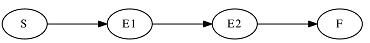
\includegraphics[width=8cm,height=1.5cm]{Simple.jpeg}
%	\label{fig:Simple}
%	\caption{}
%\end{figure}

У построенного ДКА четыре состояния: $S_{1}$ , $S_{2}$ , $S_{3}$ , $S_{4}$. Сопоставим состоянию $S_{1}$ ситуацию $E \rightarrow .E $'$+$'$ E$, $S_{2}$ ситуацию $E \rightarrow E $'$.+$'$ E$ и так далее. В итоге получим соответствие: 

\hspace{0,9cm} $S_{1}$ - $E \rightarrow .E $'$+$'$ E$

\hspace{0,9cm} $S_{2}$ - $E \rightarrow E .$'$+$'$ E$

\hspace{0,9cm} $S_{3}$ - $E \rightarrow E $'$+$'$ .E$

\hspace{0,9cm} $S_{4}$ - $E \rightarrow E $'$+$'$ E.$

Таким образом, каждой LR-ситуации мы смогли сопоставить состояние ДКА, построенного по правой части правила. Заметим, что ситуация характеризуется правилом, для которого она строится и положением точки в правой части этого правила. Теперь вернёмся к предыдущему примеру и обобщим ситуацию. 

В правой части правила - регулярное выражение. Выше мы построили по нему ДКА. Теперь построим для каждого состояния ДКА LR-ситуацию. 

Для этого сперва опишем структуру данных, в которой будем сохранять одну ситуацию. Ситуация строится для правила грамматики. Правило -- это нетерминал в левой части и ДКА, построенный по правой части. ДКА задаётся стартовым состоянием, множеством правил перехода и множеством конечных состояний. Правило перехода для ДКА -- номер текущего состояния, принимаемый символ, номер состояния, в которое переходит ДКА, приняв данный символ. Всю эту информацию необходимо хранить, для дальнейшей работы с ней. В итоге для этого потребуется структура со следующими полями:

\begin{itemize}
\item Номер правила.
\item Левая часть правила(нетерминал).
\item Номер текущего состояния ДКА.
\item Символ принимаемый ДКА в данном состоянии.  
\item Номер состояния ДКА, в которое он перейдёт приняв данный символ.
\item Номер начального состояния ДКА.
\item Номера конечных состояний ДКА.
\end{itemize}

Заметим, что эта информация состоит из двух частей: информации о ДКА в целом и правило перехода. Это ляжет в основу функции построения множества ситуаций по ДКА.

 \begin{verbatim} 
  create_items (DFA | 
 (DFA построен для правила с номером = prd_num
      и нетерминалом в левой части = prd_name )
  && (DFA = s,f,{rule | rule = (cur_num,symb,next_num)})) =
 {(prod_number,prod_name,item_number,symbol,
   next_number,start_state,finale_state)|
   prod_number = prd_num, prod_name = prd_name,
   item_number = cur_num,symbol = symb, 
   next_number = next_num,start_state = s, finale_state = f}
\end{verbatim}


\subsubsection{Вычисление GOTO}

Вычисление функции GOTO -- очень дорогая операция. При анализе вызов происходит при каждом вызове функции parse. По этому вычисление GOTO каждый раз сильно ухудшит производительность. Самое простое решение этой проблемы -- вычислить значения функции заранее, на стадии генерации данных.

На данном этапе проще всего вычислить GOTO для всех возможных пар (состояние, символ) и сконструировать коллекцию, в которой , вместо вычислений, будет производиться поиск при анализе. В качестве ключей можно взять, например, значение hash-функции от значения параметров, для которых вычислено соответствующее значение.

Основа алгоритма - стандартный алгоритм вычисления GOTO при LR анализе, подробное описание которого можно найти в ~ \cite{DrgBook}. Небольшое изменение лишь в том, что ситуация имеет специальный вид.









\subsection{���������� �������� ������}

��� ������������ ����� ���� ������ ���������� � ���, ����������� ������� ������� ������� ����� ��� ���, �� ����� �������. ������� ����� ������ ��������� - ������ ������ ������� � ������ ����������. ��� ��� ����������� ������������������� ��������, �� � ����� ������ ���� ����� ���� � ��������� �������� (����) ������. ��� ��������� ����� �������� ��� ����� ������.

����������-���������� �������� �������, ��������� ����, ����� ������� ���������� ����. ������ ���������� �������� ������� ������.

����� ������� ������ ����� �� ����� �������. ��� ����� ����������� �������� ������� \verb parse \ � \verb climb, ��������� �����.

��� ��� ���������� ������������ ��� ������ � �������������� ������������, �� � ����� ������ �� ������ ������� ��� ������. �� ���� � ������ ���� ���������� ������������ � ���������� ��������� �������� ������ ��������� ������� �������, �� ������ ���� ��������� ��� ��������� ������� ������.

������� ���������� ����������������� ������, � ����� ������� � ��������������������.

��� ����������������� �������, ���� ������� ����������� ������� �����������, ������ ���� �������� ������������ ������ ������.

�� ������ ����� ��������� ������ ����� ������� ���������� �������. ��� ������ ������� ����� ������� ������ ��� ���������������� ����������� ��� ��������� � ���������� � ��������. ��� ������������� ������ ������ ��������������� �������������� ���: 
\begin{verbatim} type tree = 
     | Node  of string*(tree list)*(string list)
     | Leaf  of string\end{verbatim}
����� ��������� �����������: $A \rightarrow R$ -- ������� ����������, ��� $A$ - ����������, $R$ - ���, ����������� �� ����������� ���������; $(A \rightarrow R,i)$ -- LR-��������, ��� $i$ - ��������� ���; $is-final(R,i)$ -- ��������, ��� $i$ - �������� ��������� $R$; $(leaf:a)$, $(A->...)$ -- ����������� ������ �������

����� ��������� ������� ����� ����� ��������� ���:

$parse$ $ q $ $ \{ u | A \rightarrow a.b, u = vx, b \rightarrow v \} \rightarrow (A \rightarrow a.b) x \{tree_i | tree_i  - $�������������� ������ ������ ��� $ t_i : t_1 .. t_n  \rightarrow \in b \})$

$climb$ $q$ $X$ $\{ u | A \rightarrow aX.b, u = vx, b \rightarrow v \} (tree: $�������������� ������ ��� X$) \rightarrow (A \rightarrow a.Xb) x \{tree_i | tree_i  - $�������������� ������ ������ ��� $ t_i : t_1 .. t_n  \rightarrow  Xb\}$

� ���� ������� ����� ��������� ���:


\verb|parse q u =|

\ \ \ \ \ \  \verb|if exists (b A| $\rightarrow$ \verb|R,i) q| \ $\&$ \ \verb|is-final(R,i)| 
  
\ \ \ \ \ \  \verb|then (A| $\rightarrow$ \verb|R,i;u;[])|

\ \ \ \ \ \  \verb|else|

\ \ \ \ \ \ \ \ \ \verb|if u=av| $\&$ \verb|exists ( A| $\rightarrow$ \verb| R,i) q* | $\&$ \verb| R(i,a)=j| 
     
\ \ \ \ \ \ \ \ \ \verb|then climb q a v (leaf:a)|
     
\ \ \ \ \ \  \verb|else|
     
\ \ \ \ \ \  \verb|if exist (A| $\rightarrow$ \verb|R,0) q*| \ $\&$ \ \verb|is-final(R,0)| 
        
        
\ \ \ \ \ \  \verb|then climb q A v (A| $\rightarrow$ \verb|[])|
        
\verb|climb q X u h = |

\ \ \ \ \ \  \verb| let (A| $\rightarrow$ \verb|R,j;w;s) = parse (goto q* X) u in|
  
  \ \ \ \ \ \ \verb| if R(i,X)=j| \ $\&$ \ \verb|(A|$\rightarrow$ \verb| R,i) in q| 
  
  \ \ \ \ \ \ \verb| then (A| $\rightarrow$ \verb| R,i;w;h::s)|
   
  \ \ \ \ \ \ \verb|else climb q A w (A| $\rightarrow$ \verb| h::s)|
  
������ ����� �������� ��� ������� ��� ������, ����� �������� ��������� �������� ������. ��� ����� ������� ��������� �������. �������, ��� ������� \verb| parse| \ � \verb| climb| \ ��� ������� ������������ ���������� �������� � �������� ��������� �� ���� ���������, � ��������� ���������. ����, ��� ����� ������ ������, � ��������, �������� ��� �� ��� � ������� ��� ������������������ �������, ������ ������������ �� ���� ���� \verb| (state,trees)| , ��� state - ��������� � trees - ��������� �������� ������, ��������������� ����� ���������, � ��������� ����� ���. ����� �������, ���������� �������� ��������� ����� \verb| (state,trees)| � �������� ��������� � �. 3.2.

����������� ������� ����������.

\hspace{0,9cm} 1) $S \rightarrow E$
 
\hspace{0,9cm} 2) $E \rightarrow E + E$

\hspace{0,9cm} 3) $E \rightarrow E * E$

\hspace{0,9cm} 4) $E \rightarrow (E)$ 

\hspace{0,9cm} 5) $E \rightarrow a$

������ ���������� ��������� �������������� ��������� � ����� ��������� ���������� � ��������.

��������, ��� ����� ���������� ������������. ���������� �������, ������� �������� ����������� ���������. ��������: ������ ������� a+a+a. ��� ����� ��� ������������� ������: 

$S\stackrel{1}{\rightarrow}E\stackrel{2}{\rightarrow}E+E \stackrel{5}{\rightarrow}a+E\stackrel{2}{\rightarrow}a+E+E\stackrel{5}{\rightarrow}a+a+E\stackrel{5}{\rightarrow}a+a+a$

�

$S\stackrel{1}{\rightarrow}E\stackrel{2}{\rightarrow}E+E \stackrel{2}{\rightarrow}E+E+E\stackrel{5}{\rightarrow}a+E+E\stackrel{5}{\rightarrow}a+a+E\stackrel{5}{\rightarrow}a+a+a$

��� �������� - ����� ������������ �� ������ ���� ������ �������.

�����, ��� ���������� ��� ������ ������� � ������ ����������:

 $(1)\rightarrow(2)\rightarrow(5)\rightarrow(2)\rightarrow(5)\rightarrow(5)$
 
 $(1)\rightarrow(2)\rightarrow(2)\rightarrow(5)\rightarrow(5)\rightarrow(5)$ 
  
 �� ������������� ������� ������:
 \clearpage
 
\begin{figure}[h]
	\centering
		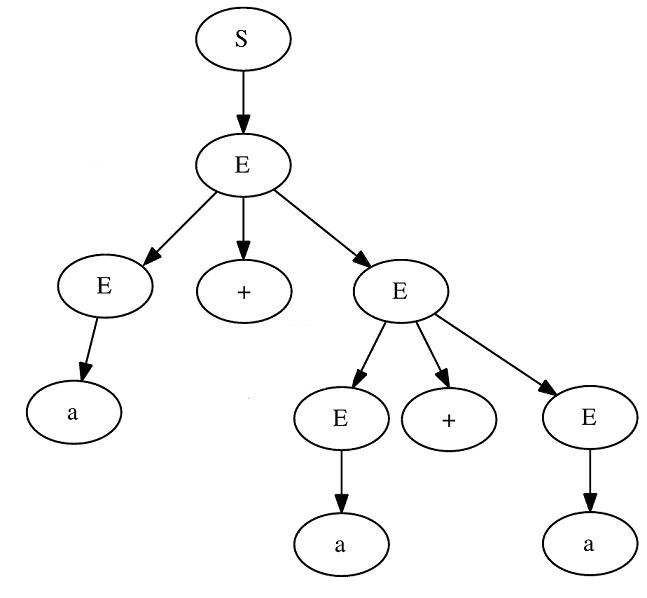
\includegraphics[width=5cm,height=6cm]{Pictures/div_tree1.jpeg}
	\label{fig:div_tree1}
\end{figure}

�

\begin{figure}[h]
	\centering
		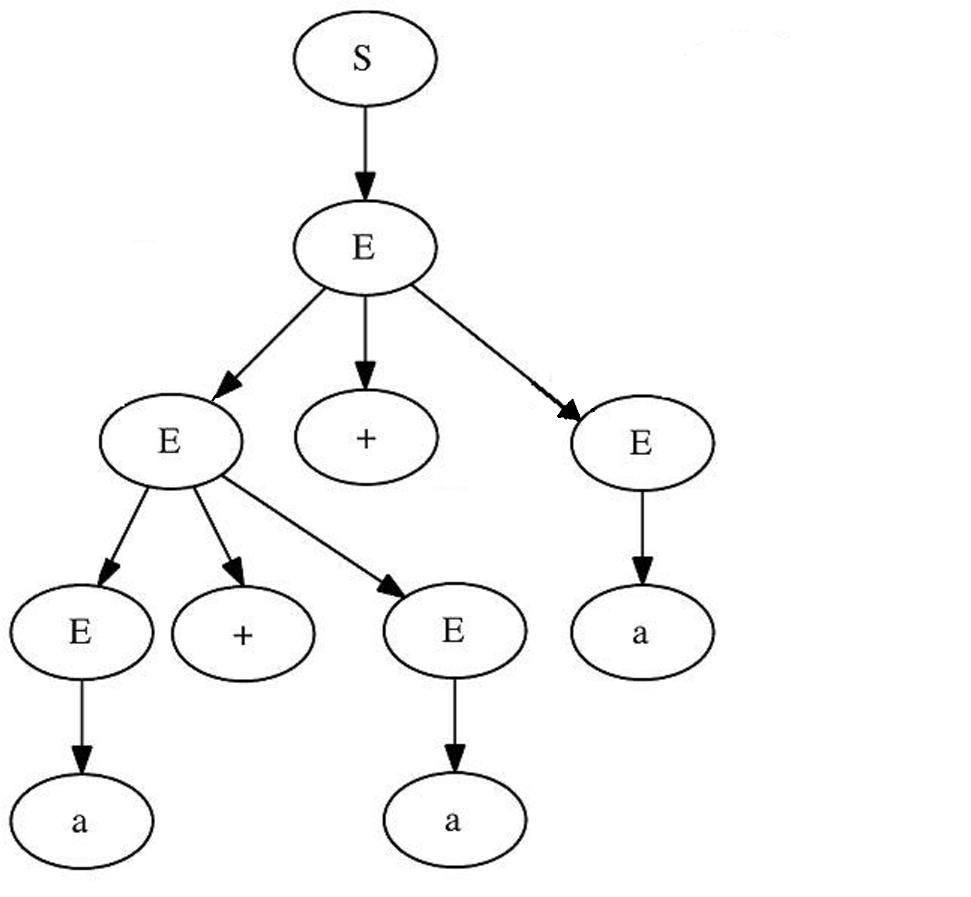
\includegraphics[width=5cm,height=6cm]{Pictures/div_tree2.jpeg}
	\label{fig:div_tree1}
\end{figure}
\clearpage
��������������, ����� �������� ��������� �������� ������, ���������� ��������� ��������� ���� ������� ���, ����� ��� ����� ����������� ��������. 
 
 

\section{Заключение}

В ходе выполнения данной дипломной работы были получены следующие результаты:
\begin{itemize}
	%\item выяснено, что предпочтительным алгоритмом анализа является GLR алгоритм;
	
	%\item изучен рекурсивно-восходящий алгоритм анализа;
	
	\item реализован прототип генератора синтаксических анализаторов со следующими свойствами:
		\begin{itemize}
		  \item принимает на вход s-атрибутную грамматику YARD-а и строит по ней транслятор
		  
			\item по однозначной LR-грамматике строится анализатор с линейной сложностью;
			
			\item по неоднозначной грамматике строится анализатор, возвращающий все возможные деревья вывода для данной входной цепочки;
			
			\item реализует поддержку EBNF-грамматик без их преобразования;
			
			\item реализует вычисление s-атрибутов; 
		
		\end{itemize}
		
\end{itemize}

Кроме того, в ходе экспериментов было выяснено, что предложенный подход, при котором явно строится лес вывода, и функции вычисления атрибутов соответствуют правилам грамматики, сильно упрощает отладку целевого инструмента.

\subsection{Дальнейшее развитие}

   Количество конструкций регулярных выражений, применяемых на практике при описании грамматики, достаточно велико, однако в инструменте поддержаны далеко не все. Ещё одним направлением развития является поддержка наследуемых атрибутов, применение которых сильно упрощает трансляцию с учётом контекста~\cite{Diploma}. Так же необходимо реализовать поддержку предикатов (резольверов~\cite{MartinenkoSUT}). Стоит отметить, что все эти возможности реализованы на уровне входного языка инструмента YARD.

Кроме того необходимо дополнить инструмент такими ставшими привычными средствами, как автоматическое восстановление от ошибок и средства диагностики ошибок.

\section{����������}
\subsection{���������� ������������� ���������� � ����������� YARD}
���� ��������� �������� ��������� ������, ��������������� ����������� ������������� ���������� � ����������� YARD, �� ����� F\# .

\begin{verbatim}
module Definition = 
  struct
    type ('patt,'expr) t = 
    { 
     head    :'expr option; 
     grammar : Grammar.t<'patt,'expr>;
     foot    :'expr option 
    }
end
\end{verbatim}

������ \verb Definition \ ������������� ����� � ��������� ����������. �������� \verb head \ � \verb foot \ ������������� ��������������� ��������� � ������ � � ����� ����� �������������. ��������, ����������� �������, �����-���� �������������� ��������, ������� ������ ���� �������� � ������� ��� "`��� ����"'.

\begin{verbatim}
module Grammar = 
  struct
    type t <'patt,'expr> = (Rule.t<'patt,'expr>) list 
  end 
\end{verbatim}

������ \verb Grammar \ -- ������������� ����������. ���������� ��� ������ ������.

\begin{verbatim}
module Rule = 
  struct
    type t <'patt,'expr> = 
    { 
     name    : string;
     args    : 'patt list;
     body    : (Production.t <'patt,'expr>);
     _public : bool; 
     metaArgs: 'patt list
    }
  end
\end{verbatim}

������ \verb Rule \ -- ������������� ������� ����������. ������� ����� ���. ��� ����� ����������� � ���������� ��� ���� ���������� (\verb adgs \ � \verb metaArgs \ ��������������). ����� �������� �� ���� ����� ������� � ������ \cite{Diploma}. ������� \verb _pablic \ ���������, �������� �� ������� ���������. � ����� ������ ����� ������ � ���������� ����� ���� ���������. ������� \verb body \ -- ������ ����� �������( ��������� ).

\begin{verbatim}
module Production = 
  struct
    type elem <'patt,'expr> = 
    {
     omit:bool; 
     rule:(t<'patt,'expr>);
     binding:'patt option; 
     checker:'expr option 
    }   
    and
    t <'patt,'expr> =    
    |PAlt     of (t <'patt,'expr>) * (t<'patt,'expr>)
    |PSeq     of (elem <'patt,'expr>) list * 'expr option 
    |PToken   of Source.t 
    |PRef     of Source.t * 'expr option // Vanilla rule reference with an optional args list.
    |PMany    of (t <'patt,'expr>) //expr*
    |PMetaRef of Source.t * 'expr option * 'expr list // Metarule reference like in "a: mr<x> y z"
    |PLiteral of Source.t 
    |PRepet   of (t <'patt,'expr>) * int option * int option  //extended regexp repetition, "man egrep" for details
    |PPerm    of (t <'patt,'expr>) list //permutation (A || B || C)
    |PSome    of (t <'patt,'expr>) //expr+
    |POpt     of (t <'patt,'expr>) //expr?

  end
\end{verbatim}

\begin{verbatim}
module Source = 
  struct
   type t = string * (int * int) 
   
   let toString ((r,_):t):string = r

  end
\end{verbatim}
\begin{thebibliography}{50}

        \bibitem {Reeng} ������������������ ������������ �������� / ��� ���. ����. �.�. �������� � �.�. ��������. - ���.: ������������ �.-�������������� ������������, 2000. 332~�.

        \bibitem {DrgBook} \emph {��� �., ���� �., ������ ��.} �����������: ��������, ����������, �����������.  �:. ������������ ��� <�������>2003. 768~�.

        \bibitem {Diploma} \emph{��������� �.�.} ��������� �������������� ������������  ��� ������� ����� ������������������� ������������� ��������. 2007. 37~c.        

        \bibitem {CCReview} \emph{��������� �.�., ������ �.�.} ����� ����������� ������� ������������� �������� �������������� ������������ // ��������� ����������������. - ���.: ���-�� �.-������. ��-��, 2006. 286-316~�.


        \bibitem {Practical Guide} \emph{Dick Grune, Ceriel Jacobs} PARSING TECHNIQUES A Practical Guide

        \bibitem {RECURSIVE-ASCENT PARSING} \emph {Larry Morell, David Middleton} RECURSIVE-ASCENT PARSING. Arkansas Tech    
                 University Russellville, Arkansas. 

        \bibitem {RecursiveAscentParsing} \emph {Lex Augusteijn} Recursive Ascent Parsing (Re: Parsing techniques). lex@prl.philips.nl (Lex Augusteijn) Mon, 10 May 1993 07:03:39 GMT 


        \bibitem {CurrentParsTechn} \emph{Mark G.J. van den Brand, Alex Sellink, Chris Verhoef} 
                Current Parsing Techniques in Software Renovation Considered Harmful.// IWPC '98: Proceedings of the 6th International Workshop on Program Comprehension. - IEEE Computer Society, Washington,1998.
        
        \bibitem {ISOEBNF} \emph ISO/IEC 14977 : 1996(E)

        \bibitem {Non-det-rec-asc} \emph {Rene Leermakers} Non-deterministic Recursive Ascent Parsing. Philips Research Laboratories,
                 P.O. Box 80.000, 5600 JA Eindhoven, The Netherlands. 

        


        \bibitem {Jade} \emph {Ronald Veldena} Jade, a recursive ascent LALR(1) parser generator. September 8,1998


        \bibitem {Bison}    http://www.gnu.org/software/bison (���� ������������� Bison)

        \bibitem {ASF+SDF}  http://www.meta-environment.org (���� ������������� ASF+SDF)

        \bibitem {.NET}     http://www.microsoft.com/NET/ (���� ��������� .NET)  

        \bibitem {FS}       http://www.research.microsoft.com/fsharp (������������ � ������������ �� ����� F\#)             

        \bibitem {Elkhound} http://www.scottmcpeak/elkhound/ (���� ������������� Elkhound )

\end{thebibliography}


\end{document}
